\section{Part II: Contributions to Language Model Alignment}

\begin{frame}[plain]
    \centering
    \vfill
    \Huge Part II\\[0.75em]\textbf{Contributions to Language Model Alignment}
    \vfill
\end{frame}

\begin{frame}{Motivation}
    \addtocounter{framenumber}{-1}
    \begin{columns}
        \begin{column}{0.5\linewidth}
            \begin{itemize}
                \item Chatbots based on Transformers~\citep{Vaswani2017attention}.
                \item Hallucinations \(\approx\) \textbf{false information}, \textbf{out of topic}, \textbf{rambling}, \textbf{toxic}...
                \item {\color{green!60!black}\textbf{Goal}}: less hallucinations.
            \end{itemize}
        \end{column}
        \begin{column}{0.5\linewidth}
            \begin{figure}
                \centering
                \includegraphics[width=\textwidth]{figures/part2/aircanada.png}
                % \caption{Air Canada's chatbot invented a refund policy while interatcing with client. [\href{URLhttps://arstechnica.com/tech-policy/2024/02/air-canada-must-honor-refund-policy-invented-by-airlines-chatbot/}{Source}]}
                \label{fig:part2:aircanada}
            \end{figure}
        \end{column}
    \end{columns}
\end{frame}

\begin{frame}{Background on Language Models}
    \begin{itemize}
        \item \textit{Vocabulary} \(\mathcal{V}\) = set of \textit{tokens} (``pieces of words'').
        \item Language model
        \begin{equation*}
           \pi_\theta : x = (\textup{token}_1, \dotsc, \textup{token}_L) \mapsto \pi_\theta (\, \cdot \, \vert x) = \text{proba. over } \mathcal{V}.
        \end{equation*}
        \item[{\color{white}\ding{118}}] {\color{white}Autoregressive generation: \textit{prompt} \(x\) \(\to\) \textit{generate} \(y\)
        \begin{align*}
            y_1 &\sim \pi_\theta (\, \cdot \, \vert x) \\
            y_2 &\sim \pi_\theta (\, \cdot \, \vert x, y_1) \\
            &\vdots \\ 
            y_t &\sim \pi_\theta (\, \cdot \, \vert x, y_{<t})
        \end{align*}}
    \end{itemize}
\end{frame}

\begin{frame}{Background on Language Models}
    \addtocounter{framenumber}{-1}
    \begin{itemize}
        \item \textit{Vocabulary} \(\mathcal{V}\) = set of \textit{tokens} (``pieces of words'').
        \item Language model
        \begin{equation*}
           \pi_\theta : x = (\textup{token}_1, \dotsc, \textup{token}_L) \mapsto \pi_\theta (\, \cdot \, \vert x) = \text{proba. over } \mathcal{V}.
        \end{equation*}
        \item Autoregressive generation: \textit{prompt} \(x\) \(\to\) \textit{response} \(y\)
        \begin{align*}
            y_1 &\sim \pi_\theta (\, \cdot \, \vert x) \\
            y_2 &\sim \pi_\theta (\, \cdot \, \vert x, y_1) \\
            &\vdots \\ 
            y_t &\sim \pi_\theta (\, \cdot \, \vert x, y_{<t})
        \end{align*}
    \end{itemize}
\end{frame}

\begin{frame}{Background on Language Models}
    \begin{itemize}
        \item \textcolor{magenta!80!black}{Pre-training}: given a dataset \(\mathcal{D}_{{\color{magenta!80!black}\textup{pre}}}\), find \(\theta\) minimizing
        \begin{equation*}
            \ell (\theta; \mathcal{D}_{{\color{magenta!80!black}\textup{pre}}}) \coloneqq - \sum_{x \in \mathcal{D}_{{\color{magenta!80!black}\textup{pre}}}} \sum_{i=1}^{\lvert x \rvert} \log{\pi_\theta \left(x_{i+1} \vert x_{\leq i} \right)}.
        \end{equation*}
        \item[{\color{white}\ding{118}}] {\color{white}\textcolor{white}{Alignment}: generate text respecting \textcolor{white}{human preferences}.}
        \item[{\color{white}\ding{118}}] {\color{white}Reinforcement learning approach:}\\[0.75em]
        \begin{enumerate}
            \item[{\color{white}1.}] {\color{white}Train a \textit{reward} model \(\textcolor{white}{R}\) on human preference data \(\mathcal{D}_{\textup{RM}}\)}
            \item[{\color{white}2.}] {\color{white}Update the \textit{writer} model \(\pi_{\textup{SFT}}\)}
        \end{enumerate}
    \end{itemize}
    \vspace{0.75em}
    {\color{white}
    \begin{equation*}
        \pi_{\color{white}\beta} \in \arg\max \, 
        \mathbb{E}_{g \sim \pi} \left[ \textcolor{white}{R(g)} \right] - \textcolor{white}{\beta} \, \textup{KL} \left( \pi \Vert \pi_{\textup{SFT}} \right)
    \end{equation*}}
\end{frame}

\begin{frame}{Background on Language Models}
    \begin{itemize}
        \item \textcolor{mygreen}{SFT}: given a \textcolor{mygreen}{task-specific} dataset \(\mathcal{D}_{{\color{mygreen}\textup{SFT}}}\), find \(\theta\) minimizing
        \begin{equation*}
            \ell (\theta; \mathcal{D}_{{\color{mygreen}\textup{SFT}}}) \coloneqq - \sum_{x \in \mathcal{D}_{{\color{mygreen}\textup{SFT}}}} \sum_{i=1}^{\lvert x \rvert} \log{\pi_\theta \left(x_{i+1} \vert x_{\leq i} \right)}.
        \end{equation*}
        \item[{\color{white}\ding{118}}] {\color{white}\textcolor{white}{Alignment}: generate text respecting \textcolor{white}{human preferences}.}
        \item[{\color{white}\ding{118}}] {\color{white}Reinforcement learning approach:}\\[0.75em]
        \begin{enumerate}
            \item[{\color{white}1.}] {\color{white}Train a \textit{reward} model \(\textcolor{white}{R}\) on human preference data \(\mathcal{D}_{\textup{RM}}\)}
            \item[{\color{white}2.}] {\color{white}Update the \textit{writer} model \(\pi_{\textup{SFT}}\)}
        \end{enumerate}
    \end{itemize}
    \vspace{0.75em}
    {\color{white}
    \begin{equation*}
        \pi_{\color{white}\beta} \in \arg\max \, 
        \mathbb{E}_{g \sim \pi} \left[ \textcolor{white}{R(g)} \right] - \textcolor{white}{\beta} \, \textup{KL} \left( \pi \Vert \pi_{\textup{SFT}} \right)
    \end{equation*}}
\end{frame}

\begin{frame}{Background on Language Models}
    \begin{itemize}
        \item \textcolor{mygreen}{SFT}: given a \textcolor{mygreen}{task-specific} dataset \(\mathcal{D}_{{\color{mygreen}\textup{SFT}}}\), find \(\theta\) minimizing
        \begin{equation*}
            \ell (\theta; \mathcal{D}_{{\color{mygreen}\textup{SFT}}}) \coloneqq - \sum_{x \in \mathcal{D}_{{\color{mygreen}\textup{SFT}}}} \sum_{i=1}^{\lvert x \rvert} \log{\pi_\theta \left(x_{i+1} \vert x_{\leq i} \right)}.
        \end{equation*}
        \item \textcolor{myorange}{Alignment}: generate text with \textcolor{myorange}{human preferences}.
        \item Reinforcement learning approach:\\[0.75em]
        \begin{enumerate}
            \item Train a \textit{reward} model \(\textcolor{myorange}{R}\) on human preference data \(\mathcal{D}_{\textup{RM}}\)
            \item Update the \textit{writer} model \(\pi_{\textup{SFT}}\)
        \end{enumerate}
    \end{itemize}
    \vspace{0.75em}
    \begin{equation*}
        \pi_{\color{myblue}\beta} \in \arg\max \, 
        \mathbb{E}_{g \sim \pi} \left[ \textcolor{myorange}{R(g)} \right] - \textcolor{myblue}{\beta} \, \textup{KL} \left( \pi \Vert \pi_{\textup{SFT}} \right)
    \end{equation*}
\end{frame}

\begin{frame}{Background on Language Models}
    \addtocounter{framenumber}{-1}
    \begin{itemize}
        \item \textcolor{mygreen}{SFT}: given a \textcolor{mygreen}{task-specific} dataset \(\mathcal{D}_{{\color{mygreen}\textup{SFT}}}\), find \(\theta\) minimizing
        \begin{equation*}
            \ell (\theta; \mathcal{D}_{{\color{mygreen}\textup{SFT}}}) \coloneqq - \sum_{x \in \mathcal{D}_{{\color{mygreen}\textup{SFT}}}} \sum_{i=1}^{\lvert x \rvert} \log{\pi_\theta \left(x_{i+1} \vert x_{\leq i} \right)}.
        \end{equation*}
        \item \textcolor{myorange}{Alignment}: generate text with \textcolor{myorange}{less hallucinations}.
        \item Reinforcement learning approach:\\[0.75em]
        \begin{enumerate}
            \item Train a \textit{reward} model \(\textcolor{myorange}{R}\) on human preference data \(\mathcal{D}_{\textup{RM}}\)
            \item Update the \textit{writer} model \(\pi_{\textup{SFT}}\)
        \end{enumerate}
    \end{itemize}
    \vspace{0.75em}
    \begin{equation*}
        \pi_{\color{myblue}\beta} \in \arg\max \, 
        \mathbb{E}_{g \sim \pi} \left[ \textcolor{myorange}{R(g)} \right] - \textcolor{myblue}{\beta} \, \textup{KL} \left( \pi \Vert \pi_{\textup{SFT}} \right)
    \end{equation*}
\end{frame}

\subsection{Reducing Hallucinations with Synthetic Hallucinations}

\begin{frame}{Research question \#1}
    \begin{itemize}
        \item[{\color{gray}\ding{118}}] {\color{gray}Reinforcement learning approach:}\\[0.75em]
        \begin{enumerate}
            \item Train a \textit{reward} model \(\textcolor{myorange}{R}\) on human preference data \(\mathcal{D}_{\textup{RM}}\)
            {\color{gray}\item[\color{gray}2.] Update the \textit{writer} model \(\pi_0\)}
        \end{enumerate}
    \end{itemize}
    \vspace{0.75em}
    {\color{gray}
    \begin{equation*}
        \pi \in \arg\max \, 
        \mathbb{E}_{g \sim \pi} \left[ R(g) \right] - \beta \, \textup{KL} \left( \pi \Vert \pi_0 \right)
    \end{equation*}
    }
    \pause
    % \vspace{1.5em}
    Getting \(\mathcal{D}_{\textup{RM}}\) is \textbf{costly}, \textbf{time-consuming}, and \textbf{error-prone}.
    \begin{tcolorbox}[colback=orange!60!white,
                    colframe=orange!60!white]
        \textbf{Research question:} \\[0.5em]
        Can synthetic hallucinations be used instead?
    \end{tcolorbox}

    \begin{itemize}
        \item Synthetic hallucinations are \textit{fast} and \textit{cheap} to implement, with \textit{automatic} and \textit{error-free} annotations.
    \end{itemize}
\end{frame}

\begin{frame}{Retrieval Augmented Generation: NPOV Task}
    \begin{figure}
        \centering
        \includegraphics[scale=0.6]{figures/part2/npov_diagram.pdf}
    \end{figure}
\end{frame}

\begin{frame}{Creating Synthetic Hallucinations}
\textcolor{mygreen}{Pros:}
\begin{enumerate}
    \item[{\color{mygreen}1.}] \textcolor{mygreen}{Studies show marijuana is a safe drug}
    \item[{\color{mygreen}2.}] \textcolor{mygreen}{Legalization boosts the economy}
\end{enumerate}
{\color{myblue}
Cons:}
\begin{enumerate}
    \item[{\color{myblue}1.}] \textcolor{myblue}{Marijuana is a gateway drug}
    \item[{\color{myblue}2.}] \textcolor{myblue}{Legalization brings costs}
\end{enumerate}
\vspace{0.75em}
\textit{Neutral answer:}\\[0.75em]   
``Some people support marijuana legalization because {\color{mygreen}it would boost the economy} and {\color{mygreen}most studies demonstrate it is a safe drug}. Others oppose it because they see {\color{myblue}marijuana as a gateway drug}, and its {\color{myblue}legalization would bring many costs}.''
\end{frame}

\begin{frame}{Creating Synthetic Hallucinations}
\textcolor{mygreen}{Pros:}
\begin{enumerate}
    \item[{\color{mygreen}1.}] \textcolor{mygreen}{Studies show marijuana is a safe drug}
    \item[{\color{mygreen}2.}] \textcolor{mygreen}{Legalization boosts the economy}
\end{enumerate}
{\color{myblue}
Cons:}
\begin{enumerate}
    \item[{\color{myblue}1.}] \textcolor{myblue}{\st{Marijuana is a gateway drug}}
    \item[{\color{myblue}2.}] \textcolor{myblue}{Legalization brings costs}
\end{enumerate}
\vspace{0.75em}
\textit{Neutral answer:}\\[0.75em]   
``Some people support marijuana legalization because {\color{mygreen}it would boost the economy} and {\color{mygreen}most studies demonstrate it is a safe drug}. Others oppose it because they see \mycolorbox{red!70!white}{marijuana as a} \mycolorbox{red!70!white}{gateway drug}, and its {\color{myblue}legalization would bring many costs}.''
\end{frame}

% \begin{frame}{Results}
%     \begin{figure}[h]
%     \centering
%     % Define 3 columns:
%     % 1st column: for the Row Labels (e.g., 2.5cm wide, centered)
%     % 2nd and 3rd columns: for the Images (p-type for alignment)
%     \begin{tabular}{c p{0.48\textwidth} p{0.48\textwidth}} 
    
%         % --- Row 1: Column Labels ---
%         % The first cell is empty, the next two are the column titles
%         & \multicolumn{1}{c}{\textbf{Condition A}} & \multicolumn{1}{c}{\textbf{Condition B}} \\
        
%         % --- Row 2: Row Label + Images ---
%         \multicolumn{1}{c}{\textbf{\rotatebox{90}{Experiment 1}}} & 
%         \includegraphics[width=\textwidth]{figures/part2/npov_rm_organic.png} &
%         \includegraphics[width=\textwidth]{figures/part2/npov_rm_struct.png} \\
        
%         % --- Row 3: Row Label + Images ---
%         \multicolumn{1}{c}{\textbf{\rotatebox{90}{Experiment 2}}} & 
%         \includegraphics[width=\textwidth]{figures/part2/npov_perl_organic_reward.png} &
%         \includegraphics[width=\textwidth]{figures/part2/npov_perl_struct_reward.png} \\
        
%     \end{tabular}
%     \caption{A $2 \times 2$ image grid showing results under different conditions.}
%     \label{fig:2x2_labeled_grid}
% \end{figure}
% \end{frame}

\begin{frame}{Results}
\centering

\begin{table}[h]
    \footnotesize
    \centering
    \begin{tabular}{ccc}
    \toprule
    \textit{SFT baseline} (\%) & \textit{Organic hallucinations} (\%) & \textit{Synthetic hallucinations} (\%) \\
    \midrule
    10.2 & 3.0 & 0.74 \\
    \bottomrule
    \end{tabular}
    \label{tab:npov_results}
\end{table}

% Adjust total width to something safely below slide width
\newlength{\imgw}
\setlength{\imgw}{0.28\textwidth} % tweak if needed

\begin{tabular}{c c c}
    % Column titles
    & \textbf{Organic} & \textbf{Synthetic} \\

    % Row 1
    \rotatebox{90}{\hspace{0.2cm}\textbf{RM ROC-AUC}} &
    \includegraphics[width=\imgw]{figures/part2/npov_rm_organic.png} &
    \includegraphics[width=\imgw]{figures/part2/npov_rm_struct.png} \\

    % Row 2
    \rotatebox{90}{\hspace{0.5cm}\textbf{RL scores}} &
    \includegraphics[width=\imgw]{figures/part2/npov_perl_organic_reward.png} &
    \includegraphics[width=\imgw]{figures/part2/npov_perl_struct_reward.png} \\
\end{tabular}
\end{frame}

\begin{frame}{Discussion}
    \begin{itemize}
        \item \textbf{Code}: \url{github.com/leobianco/perl_hallucination}
    \end{itemize}
    \vspace{0.75em}
    Future work:
    \vspace{0.75em}
    \begin{itemize}
        \item Other task (summarization).
        \item Other models (Mistral, Qwen).
        \item Other synthetic hallucinations schemes (LLM).
    \end{itemize}
\end{frame}

\subsection{Decoding-time Realignment of Language Models}

\begin{frame}{Research question \#2}
    \begin{itemize}
        \item[{\color{gray}\ding{118}}] {\color{gray}Reinforcement learning approach:}\\[0.75em]
        \begin{enumerate}
            {\color{gray}\item[\color{gray}1.] Train a \textit{reward} model \(R\) on human preference data \(\mathcal{D}_{\textup{RM}}\)}
            \item[2.] Update the \textit{writer} model \(\pi_0\)
        \end{enumerate}
    \end{itemize}
    \vspace{0.75em}
    \begin{equation*}
        \pi_{\color{myblue}\beta} \in \arg\max \, 
        \mathbb{E}_{g \sim \pi} \left[ \textcolor{myorange}{R(g)} \right] - \textcolor{myblue}{\beta} \, \textup{KL} \left( \pi \Vert \pi_{\textup{SFT}} \right)
    \end{equation*}
    \pause
    The hyperparameter \(\textcolor{myblue}{\beta}\) is expensive to tune via grid-search.
    \begin{tcolorbox}[colback=orange!60!white,
                    colframe=orange!60!white]
        \textbf{Research question:} \\[0.5em]
        Can we adjust regularization strength without retraining?
    \end{tcolorbox}
\end{frame}

\begin{frame}{Results}
    \begin{itemize}
        \item \textbf{Contribution}: approximate realigned model at \(\beta / \lambda\)
    \end{itemize}
    \begin{tcolorbox}[colback=yellow!45!white, colframe=yellow!45!white]
        \begin{equation*}
            \hat{\pi}_{\beta/\lambda} (\, \cdot \, \vert x, y_{<t}) \coloneqq \textup{softmax} \left[ \lambda h_\beta^{(t)} + (1 - \lambda) h_{\textup{SFT}}^{(t)} \right]
        \end{equation*}
    \end{tcolorbox}
    \begin{itemize}
        \item[] where \(h^{(t)}_{\textup{SFT}}\) and \(h^{(t)}_{\beta}\) are the logits 
        \begin{align*}
            \begin{cases}
                \pi_{\textup{SFT}} (\, \cdot \, \vert x, y_{< t}) &= \textup{softmax} (h^{(t)}_{\textup{SFT}}) \\[0.75em]
                \pi_{\beta} (\, \cdot \, \vert x, y_{< t}) &= \textup{softmax} (h^{(t)}_{\beta})
            \end{cases}
        \end{align*}
    \end{itemize}
    \begin{itemize}
        \item \textbf{Code}: \url{https://github.com/liutianlin0121/decoding-time-realignment}
    \end{itemize}
\end{frame}

\begin{frame}{Results}
    \begin{figure}
        \centering
        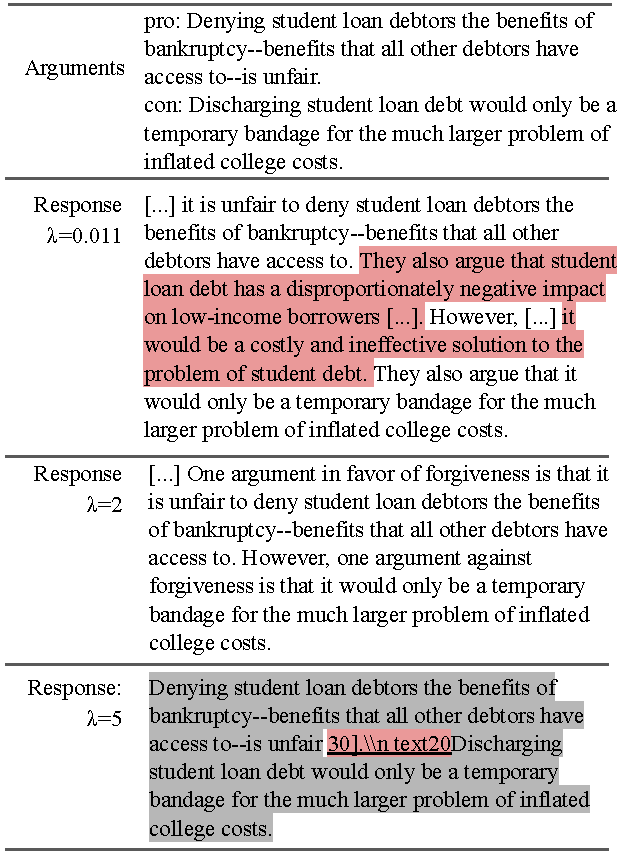
\includegraphics[scale=0.55]{figures/part2/dera-hallucination-single-col.pdf}
    \end{figure}
\end{frame}

\begin{frame}{Results}
    \begin{figure}
        \centering
        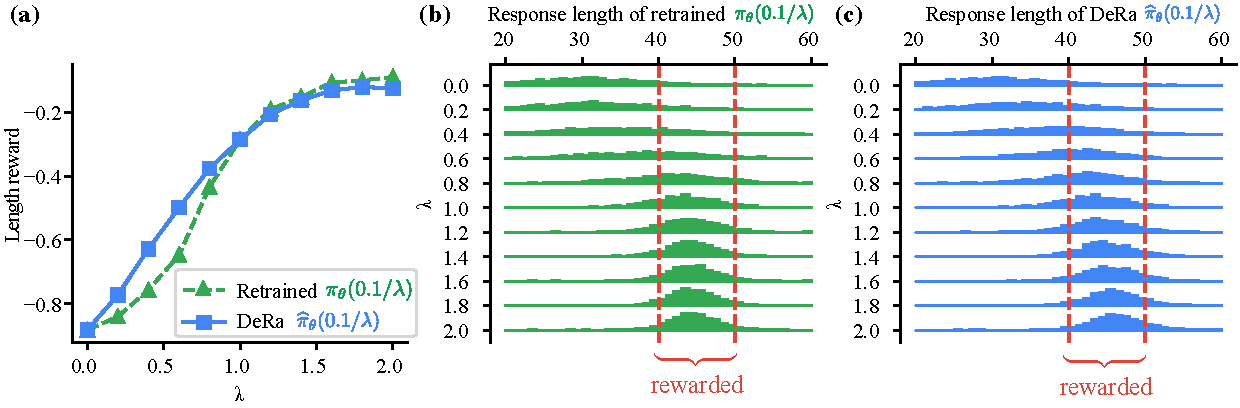
\includegraphics[scale=0.5]{figures/part2/length_reward_result_no_sax.pdf}
    \end{figure}
\end{frame}

\begin{frame}{Discussion}
    \begin{itemize}
        \item ?
    \end{itemize}
    
\end{frame}
